% This file was created with tikzplotlib v0.10.1.
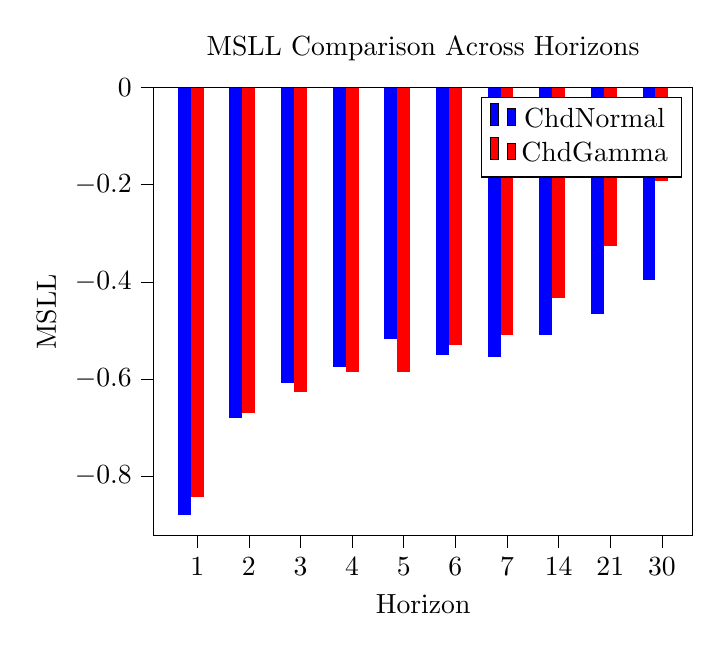
\begin{tikzpicture}

\definecolor{darkgray176}{RGB}{176,176,176}

\begin{axis}[
tick align=outside,
tick pos=left,
title={MSLL Comparison Across Horizons},
x grid style={darkgray176},
xlabel={Horizon},
xmin=-0.85, xmax=9.6,
xtick style={color=black},
xtick={0,1,2,3,4,5,6,7,8,9},
xticklabels={1,2,3,4,5,6,7,14,21,30},
y grid style={darkgray176},
ylabel={MSLL},
ymin=-0.923060773977745, ymax=0,
ytick style={color=black}
]
\draw[draw=none,fill=blue] (axis cs:-0.375,0) rectangle (axis cs:-0.125,-0.879105499026424);
\addlegendimage{ybar,ybar legend,draw=none,fill=blue}
\addlegendentry{ChdNormal}

\draw[draw=none,fill=blue] (axis cs:0.625,0) rectangle (axis cs:0.875,-0.681191498170826);
\draw[draw=none,fill=blue] (axis cs:1.625,0) rectangle (axis cs:1.875,-0.607558924593337);
\draw[draw=none,fill=blue] (axis cs:2.625,0) rectangle (axis cs:2.875,-0.57495648241054);
\draw[draw=none,fill=blue] (axis cs:3.625,0) rectangle (axis cs:3.875,-0.517959518063628);
\draw[draw=none,fill=blue] (axis cs:4.625,0) rectangle (axis cs:4.875,-0.550090004032213);
\draw[draw=none,fill=blue] (axis cs:5.625,0) rectangle (axis cs:5.875,-0.554156438489196);
\draw[draw=none,fill=blue] (axis cs:6.625,0) rectangle (axis cs:6.875,-0.509945837690314);
\draw[draw=none,fill=blue] (axis cs:7.625,0) rectangle (axis cs:7.875,-0.466212819953932);
\draw[draw=none,fill=blue] (axis cs:8.625,0) rectangle (axis cs:8.875,-0.395250514083511);
\draw[draw=none,fill=red] (axis cs:-0.125,0) rectangle (axis cs:0.125,-0.84283760634468);
\addlegendimage{ybar,ybar legend,draw=none,fill=red}
\addlegendentry{ChdGamma}

\draw[draw=none,fill=red] (axis cs:0.875,0) rectangle (axis cs:1.125,-0.670576250873894);
\draw[draw=none,fill=red] (axis cs:1.875,0) rectangle (axis cs:2.125,-0.627384887140095);
\draw[draw=none,fill=red] (axis cs:2.875,0) rectangle (axis cs:3.125,-0.585345420276347);
\draw[draw=none,fill=red] (axis cs:3.875,0) rectangle (axis cs:4.125,-0.585796380115982);
\draw[draw=none,fill=red] (axis cs:4.875,0) rectangle (axis cs:5.125,-0.530099229753413);
\draw[draw=none,fill=red] (axis cs:5.875,0) rectangle (axis cs:6.125,-0.508665713685634);
\draw[draw=none,fill=red] (axis cs:6.875,0) rectangle (axis cs:7.125,-0.433929896488731);
\draw[draw=none,fill=red] (axis cs:7.875,0) rectangle (axis cs:8.125,-0.326009718113609);
\draw[draw=none,fill=red] (axis cs:8.875,0) rectangle (axis cs:9.125,-0.19145729323947);
\end{axis}

\end{tikzpicture}
